\chapter{Desenvolvimento elétrico e eletrônico}\label{cap:eletrica}
A organização elétrica acompanha a divisão modular do aparelho. A central distribui alimentação e coordena o barramento; o intermediário controla a sinalização; e o submódulo reúne o acionamento e a leitura óptica. O projeto separa os ramais de potência de 5 V da lógica de 3,3 V e mantém referência de terra comum.

\section{Distribuição da alimentação}
Foi prevista uma fonte regulada de 5 V com capacidade nominal de 10 A. A distribuição utiliza ramais para a Raspberry Pi, o buzzer e a cadeia de módulos. No submódulo, a alimentação atende à ESP32 e à placa de acionamento do motor, enquanto o circuito óptico utiliza a referência de 3,3 V. A Figura~\ref{fig:distribuicao_alimentacao} apresenta a organização funcional. \cite{DC_CIRCUITOS}

\begin{figure}[htbp]
\centering
\caption{Distribuição funcional da alimentação de 5 V e da referência comum}\label{fig:distribuicao_alimentacao}
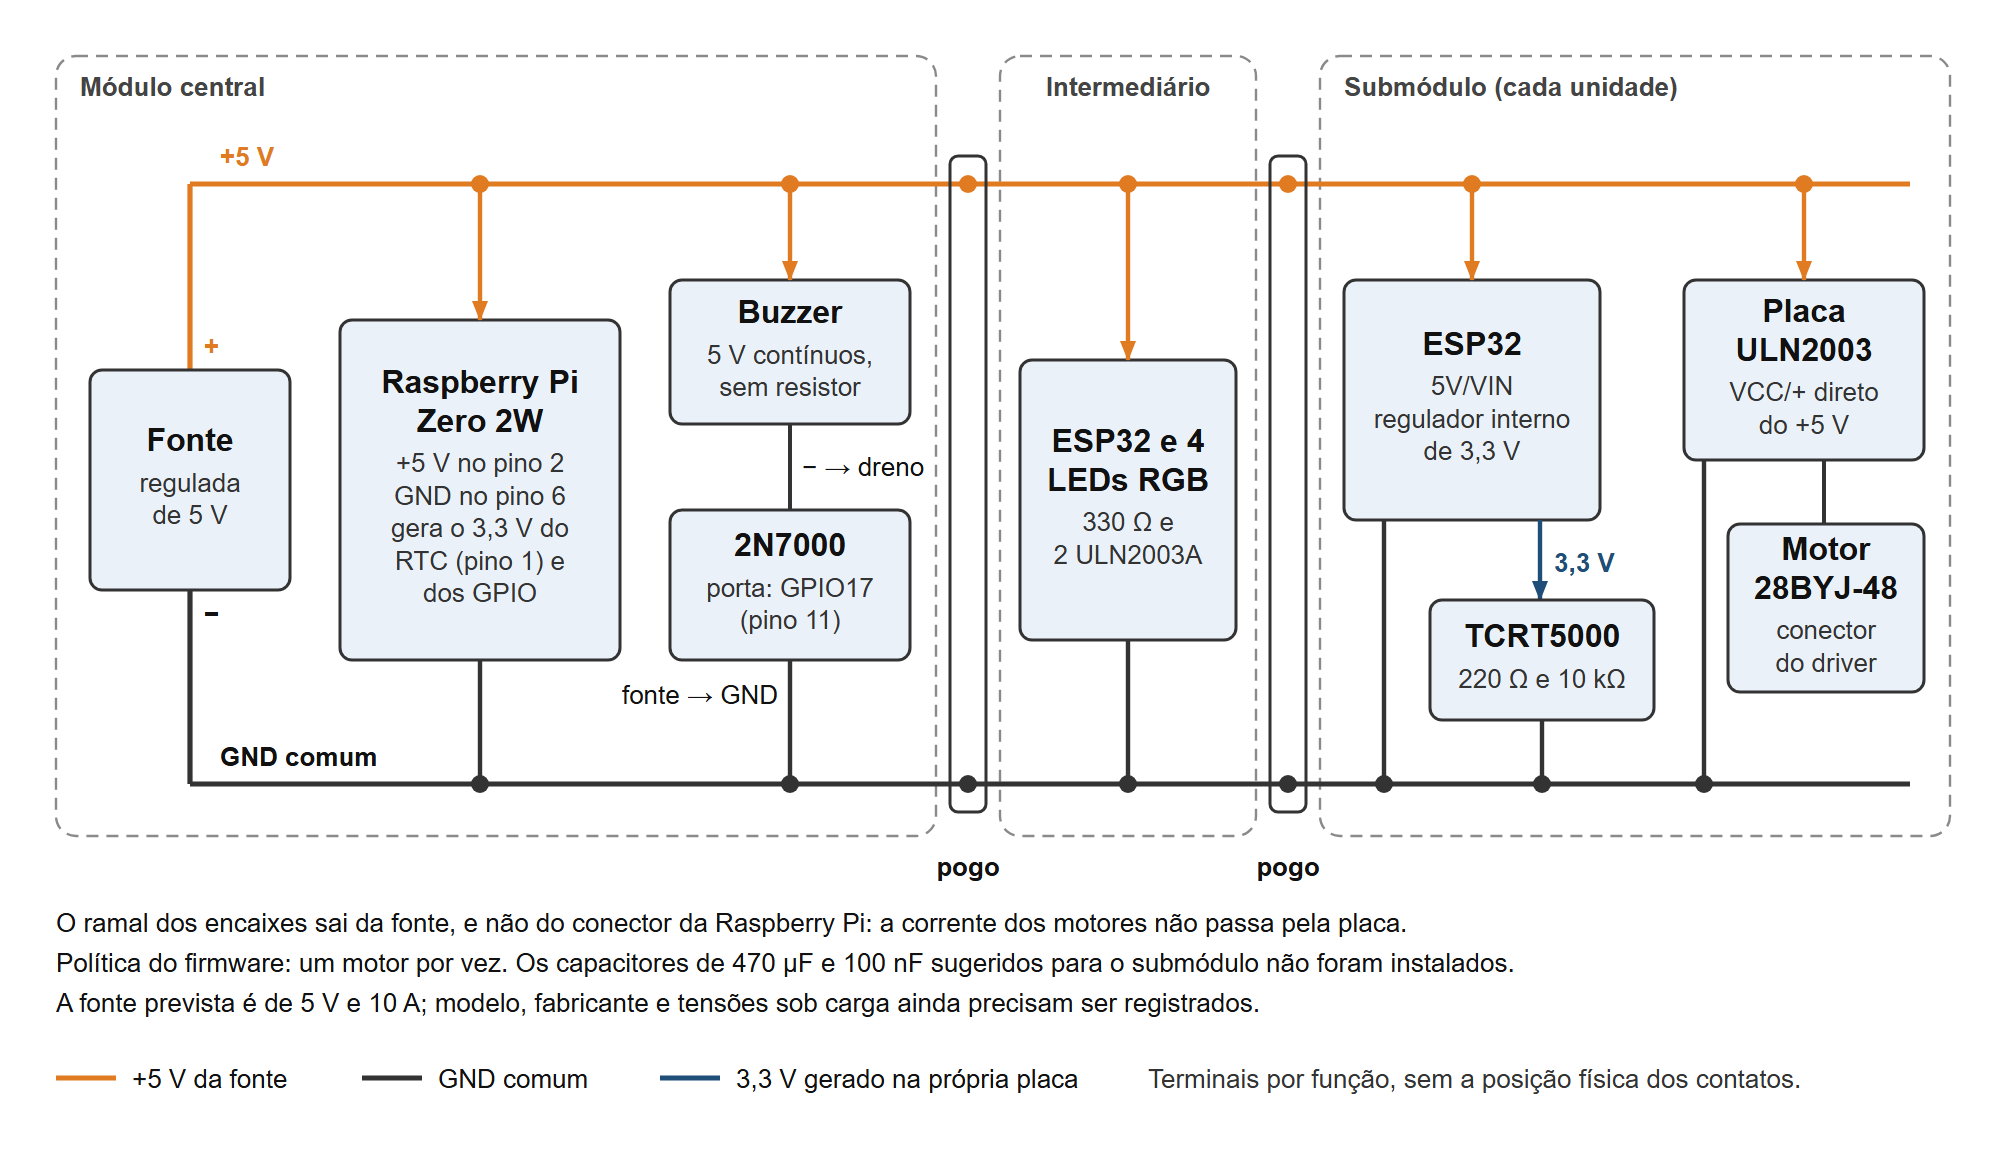
\includegraphics[width=0.98\textwidth,height=0.66\textheight,keepaspectratio]{Figuras/SharePoint/distribuicao_alimentacao.png}
\fonte{Elaboração dos autores (2026).}
\end{figure}


A corrente nominal da fonte não corresponde ao consumo do aparelho. A avaliação do fornecimento considera queda de tensão e corrente durante repouso, comunicação e atuação. O retorno comum também precisa manter referência adequada entre os sinais, evitando que o acionamento do motor comprometa as leituras e o barramento.

\section{Unidade central}
A Raspberry Pi Zero 2 W utiliza GPIO2 para SDA e GPIO3 para SCL, com lógica de 3,3 V. A central também reúne o módulo de relógio HW-084 com DS3231M, o buzzer e os sinais luminosos. Na coleta de 26 de novembro, o RTC não estava ativado no Linux; o tempo confiável dependia da rede. A presença de bateria compatível ainda precisava ser conferida. \cite{DC_VALIDACAO2026} A Figura~\ref{fig:circuito_central} apresenta as ligações por função. A interface de quatro vias deve ser identificada por continuidade, pois uma relação textual de sinais não determina sua ordem física no conector.

\begin{figure}[htbp]
\centering
\caption{Ligações funcionais da unidade central}\label{fig:circuito_central}
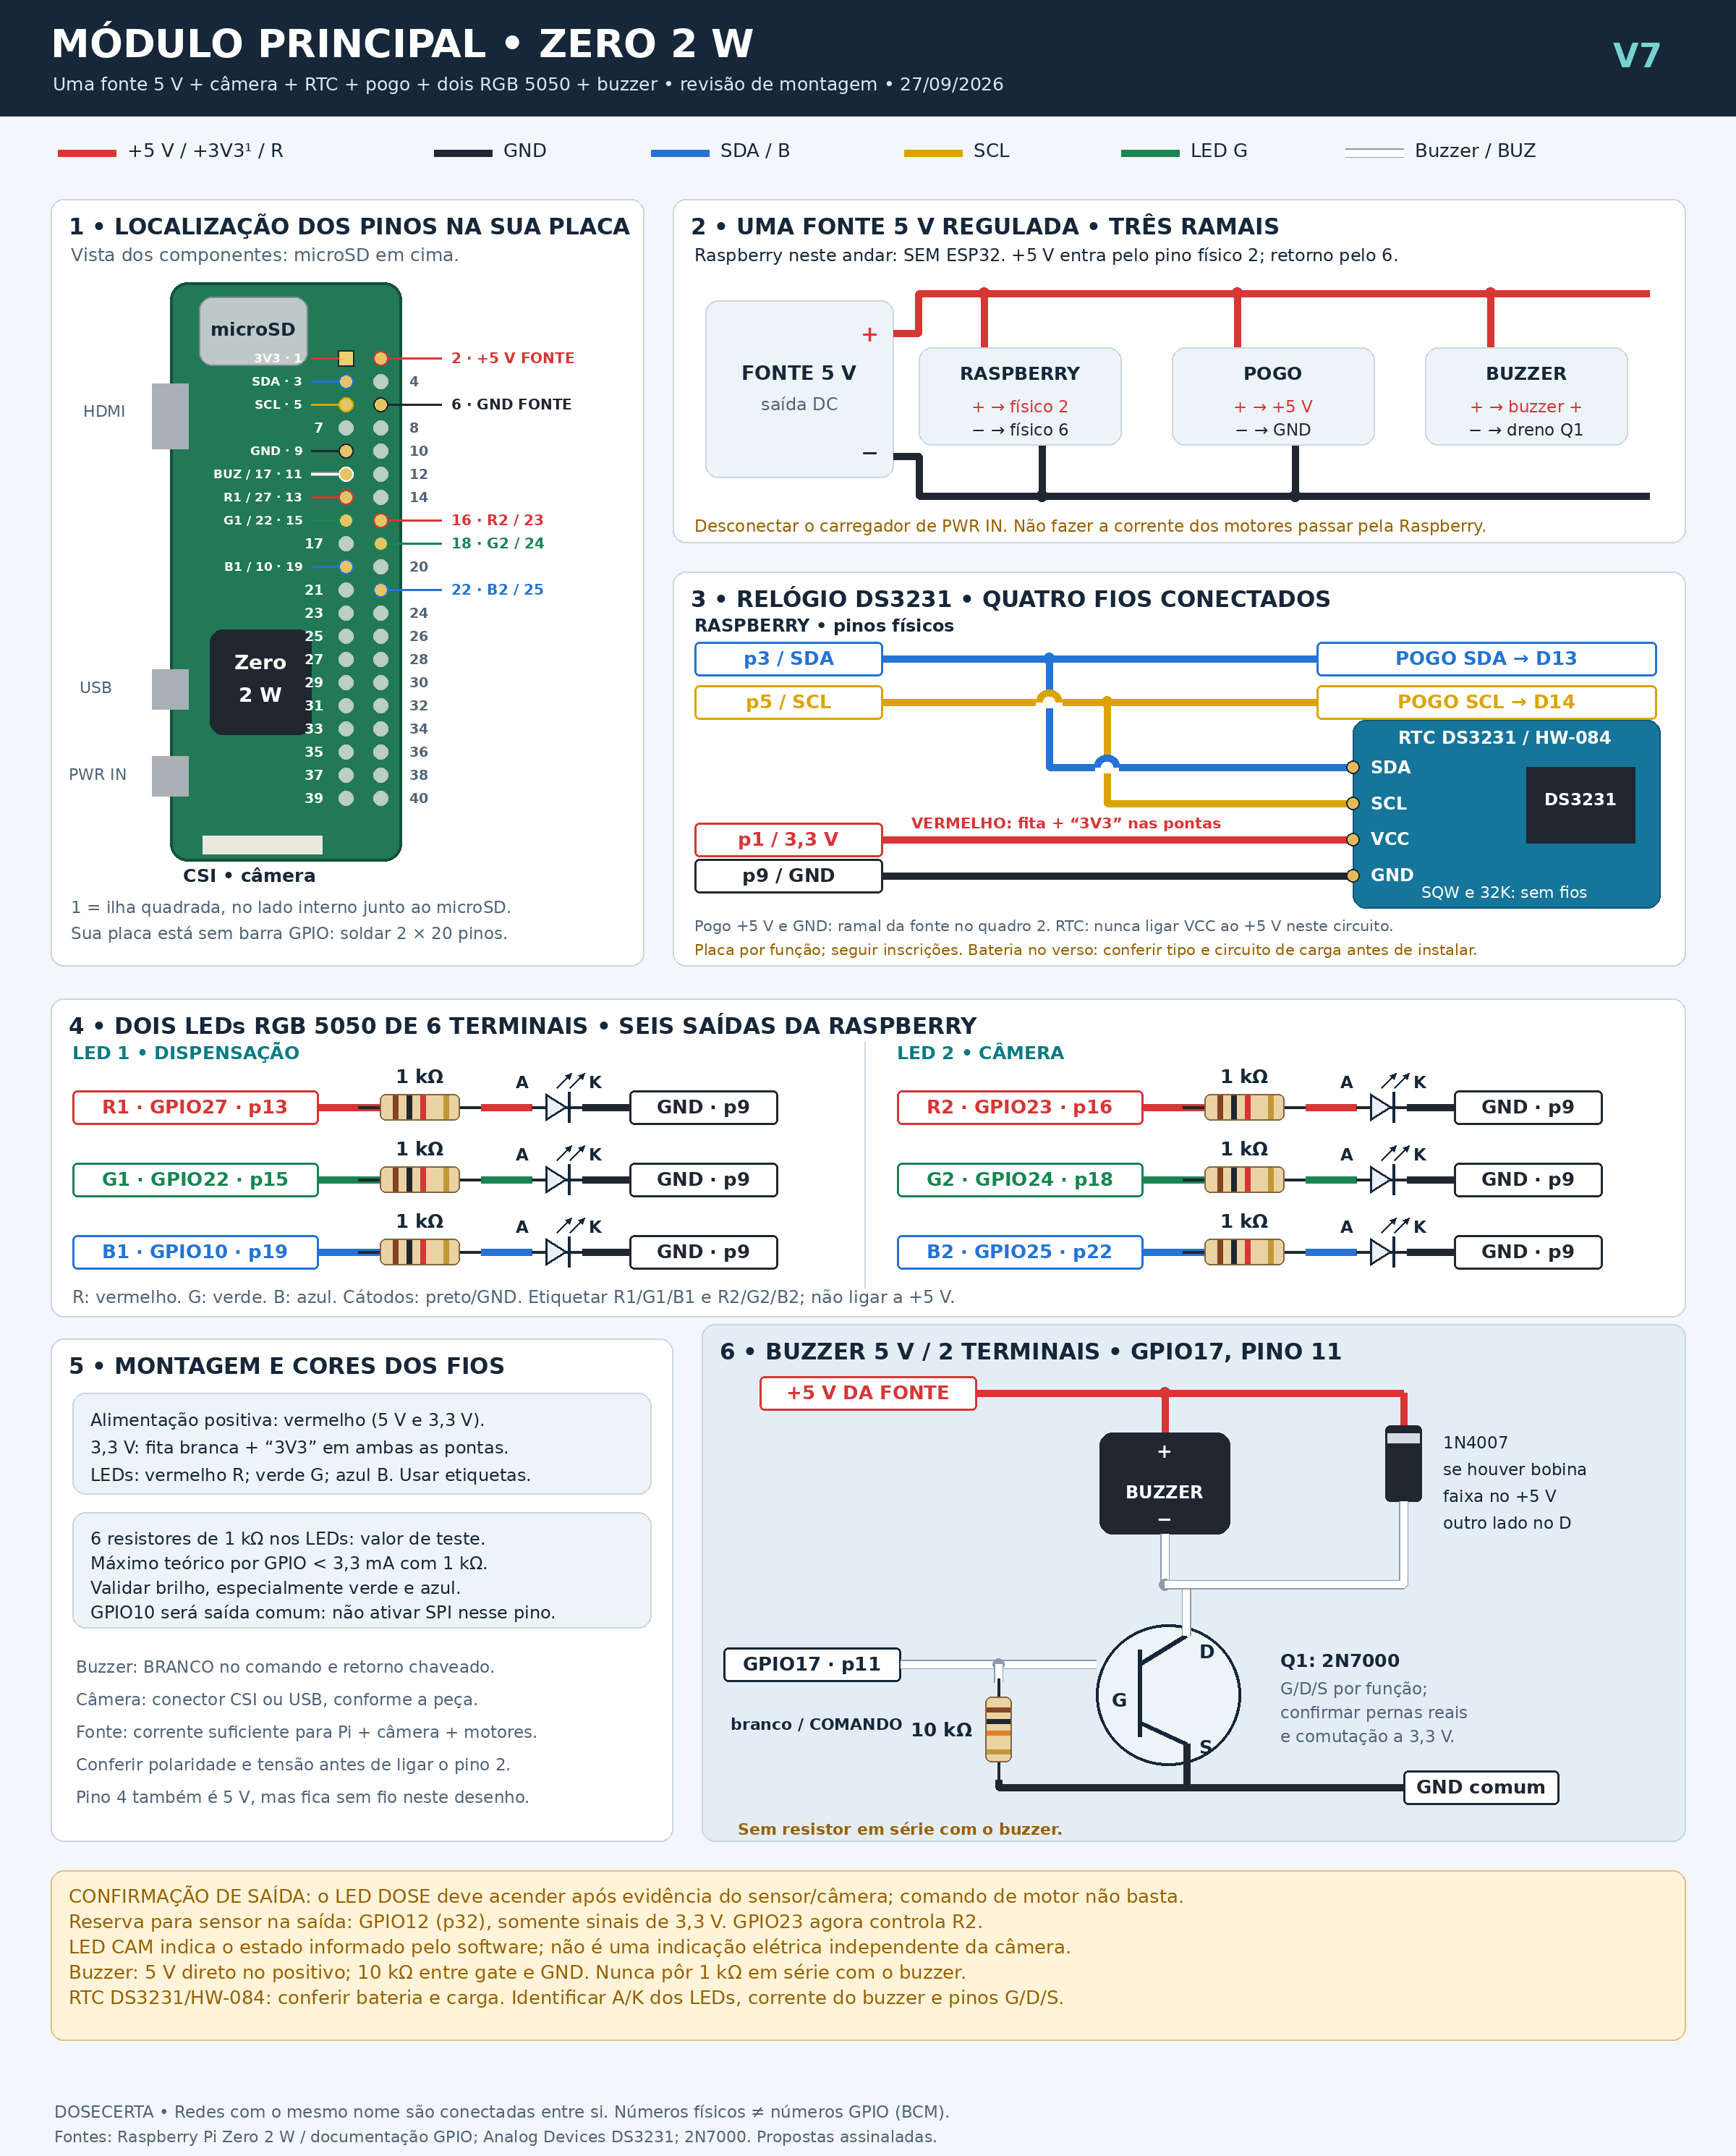
\includegraphics[width=0.98\textwidth,height=0.73\textheight,keepaspectratio]{Figuras/SharePoint/circuito_central.png}
\fonte{Elaboração dos autores (set. 2026). Distribuição funcional, sem definição da ordem física dos contatos.}
\end{figure}


O buzzer é alimentado pelo ramal de 5 V e chaveado pelo transistor 2N7000. O GPIO17 atua na porta, e o resistor de 10 k\ensuremath{\Omega} entre porta e fonte mantém a condição de desligamento. A Figura~\ref{fig:buzzer} detalha esse estágio. A identificação dos terminais e a condução com 3,3 V devem ser conferidas para o componente instalado.

\begin{figure}[htbp]
\centering
\caption{Estágio de acionamento do buzzer com transistor 2N7000}\label{fig:buzzer}
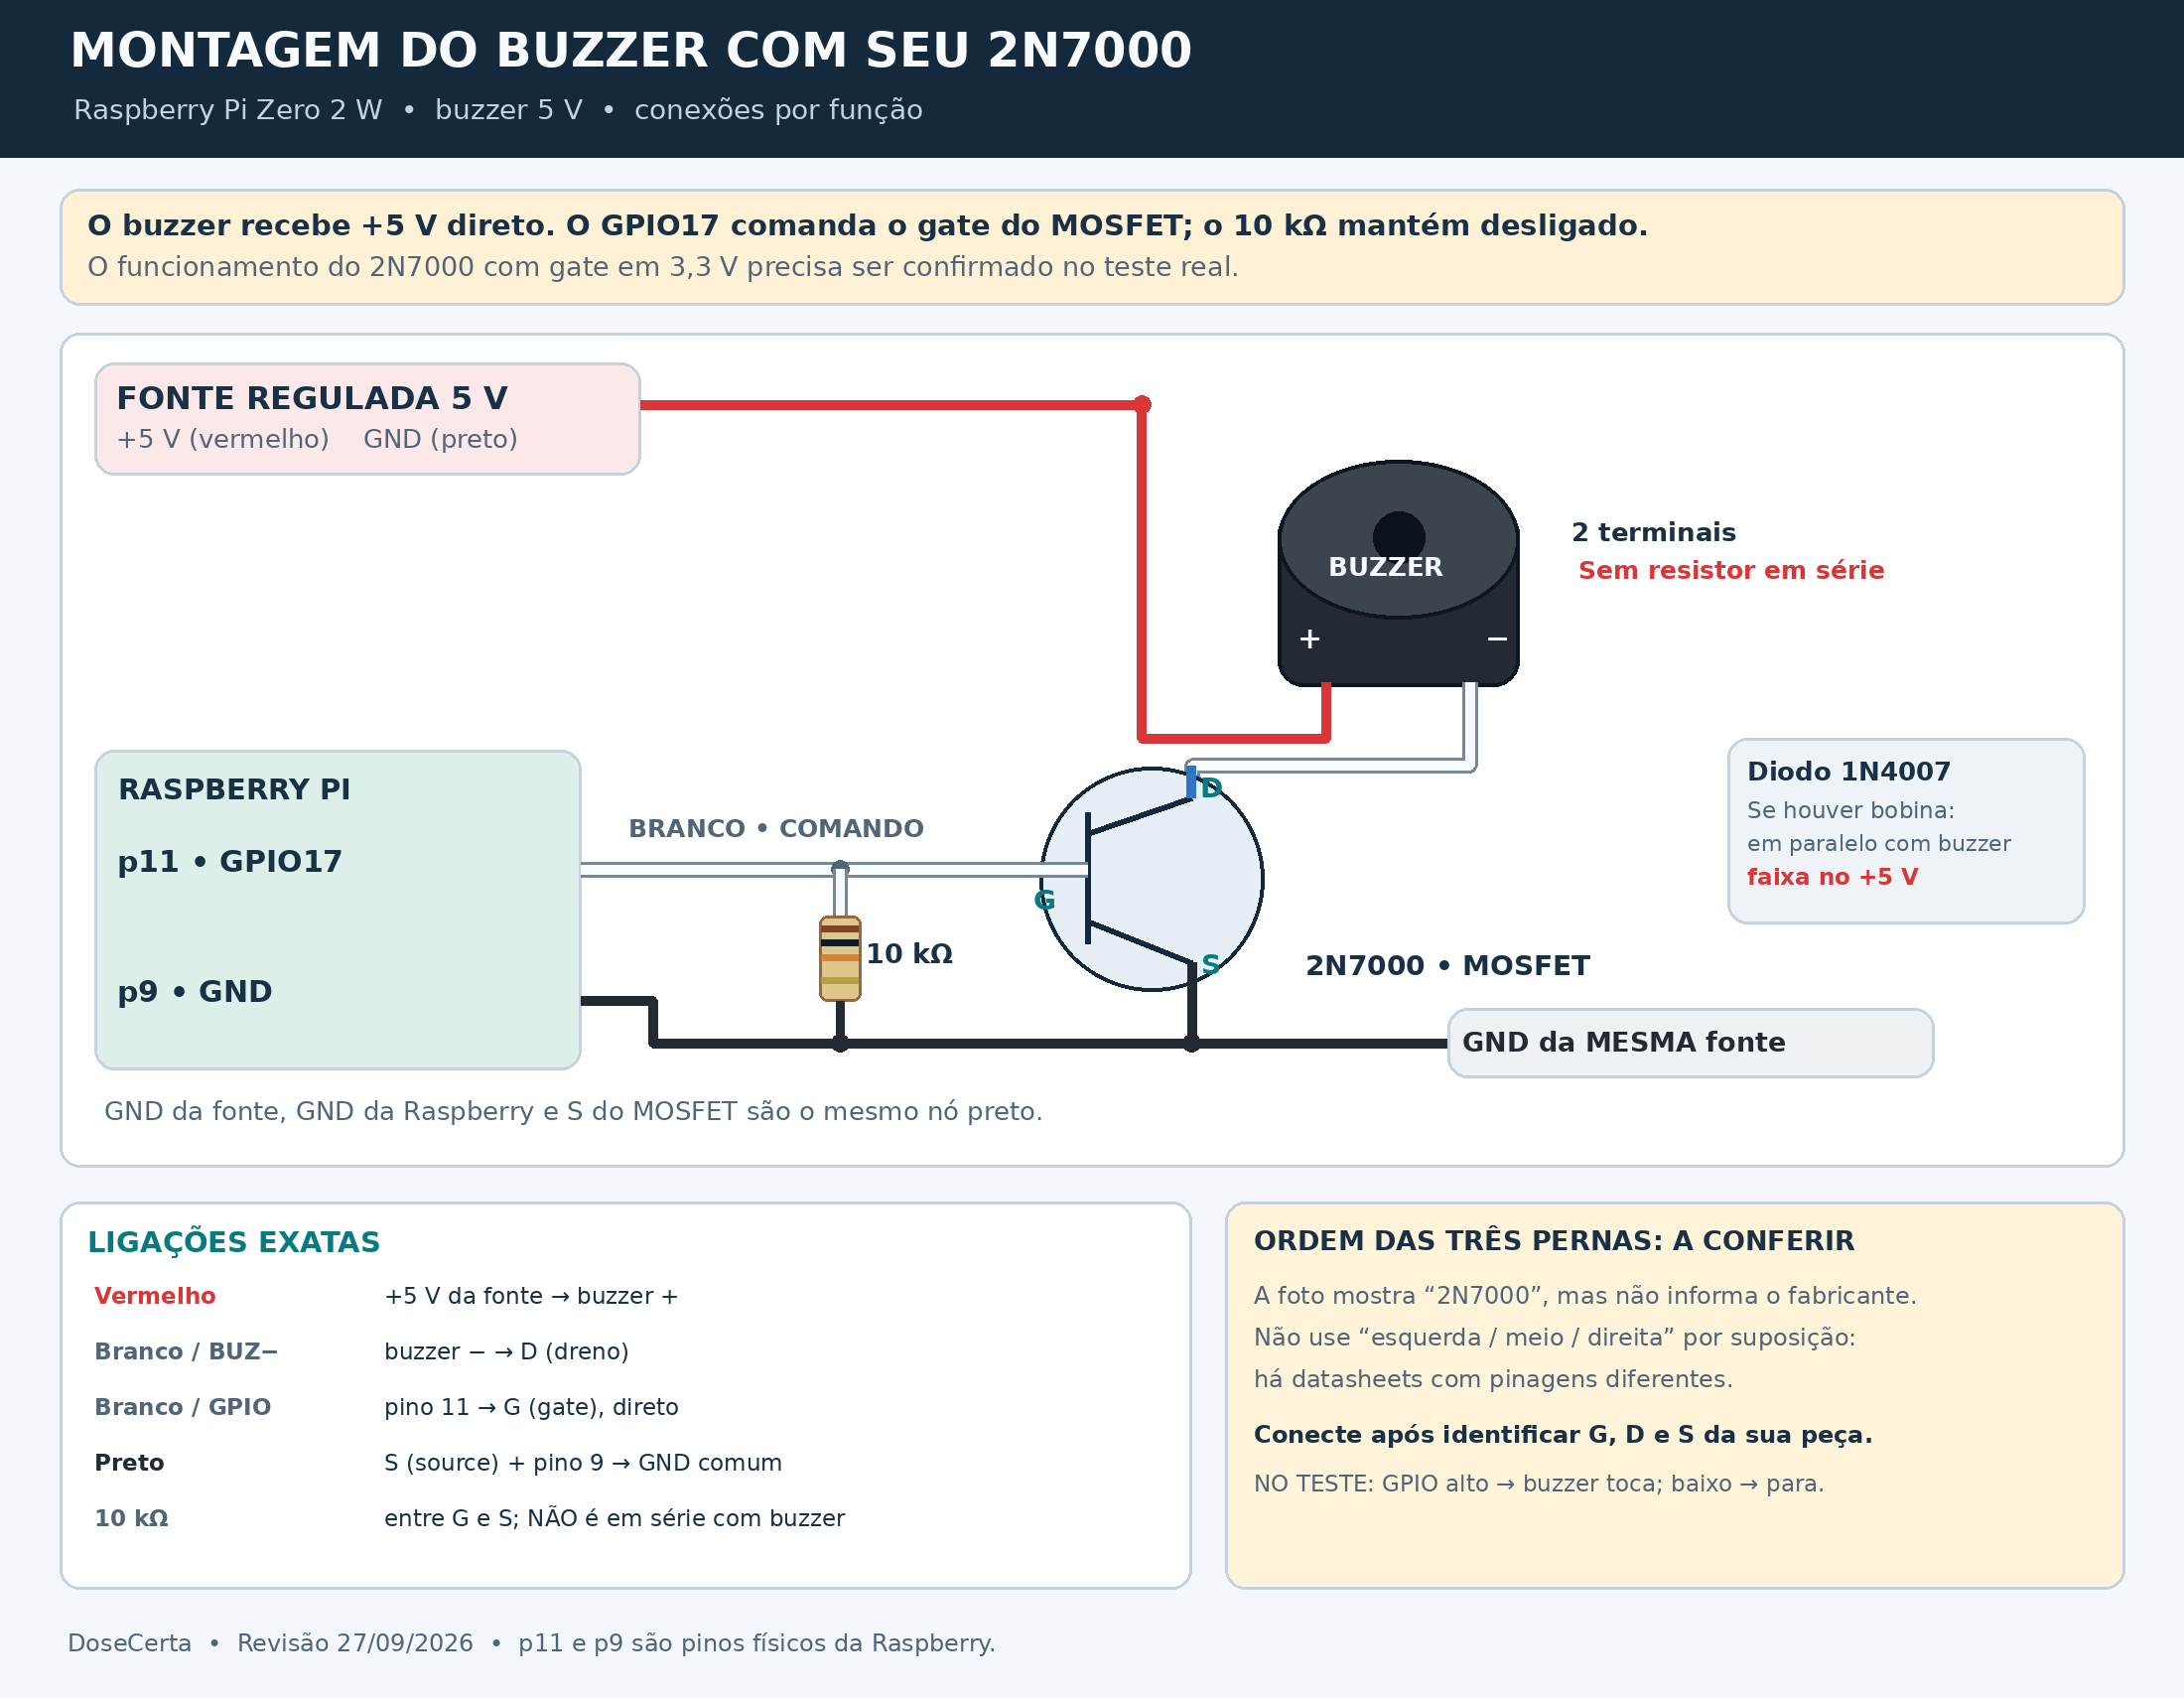
\includegraphics[width=0.91\textwidth,height=0.66\textheight,keepaspectratio]{Figuras/SharePoint/buzzer.png}
\fonte{Elaboração dos autores (set. 2026). Terminais e condição de acionamento dependem da peça utilizada.}
\end{figure}


\section{Submódulo dosador}
No submódulo, a ESP32 controla o 28BYJ-48 por meio da placa ULN2003 e lê o TCRT5000 no ADC1. Os sinais do motor utilizam GPIO27, GPIO26, GPIO25 e GPIO33, e a leitura óptica utiliza GPIO32. O barramento chega aos GPIO13 e GPIO14. A Figura~\ref{fig:circuito_submodulo} reúne essas ligações.

\begin{figure}[htbp]
\centering
\caption{Ligações funcionais do submódulo dosador}\label{fig:circuito_submodulo}
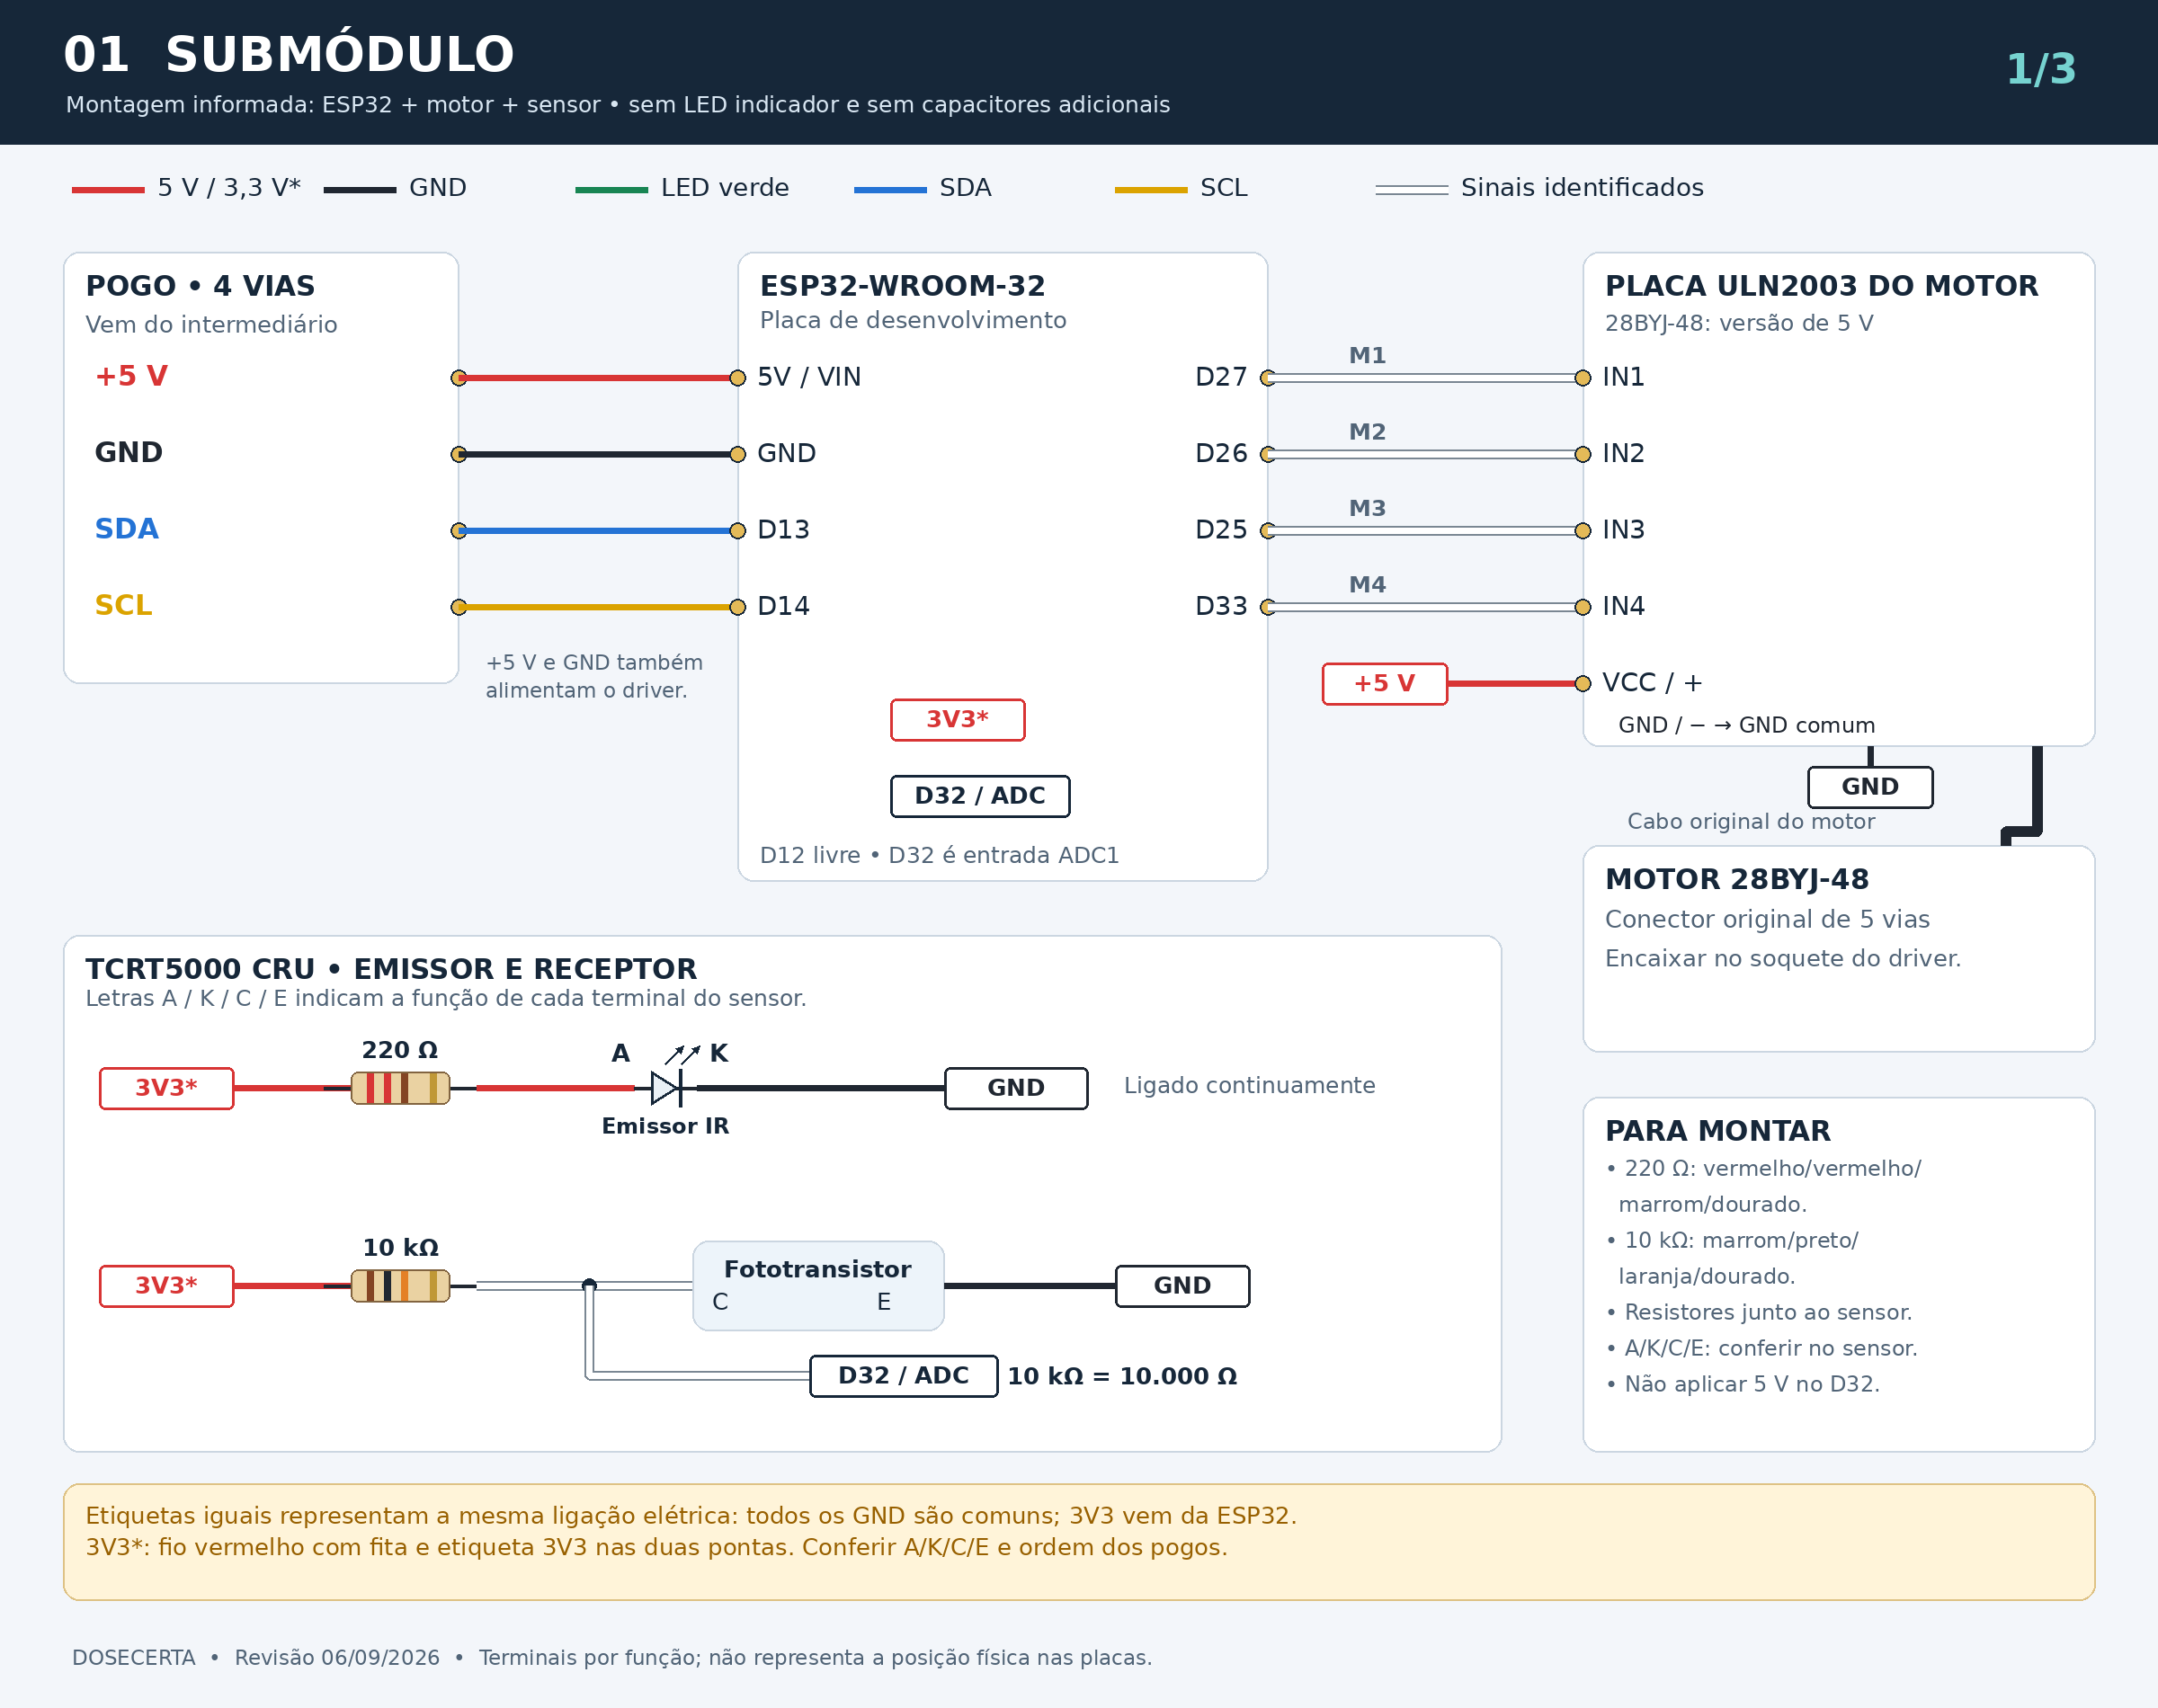
\includegraphics[width=0.98\textwidth,height=0.70\textheight,keepaspectratio]{Figuras/SharePoint/circuito_submodulo.png}
\fonte{Elaboração dos autores (set. 2026). Prancha anterior às correções finais de bancada.}
\end{figure}


O emissor infravermelho utiliza resistor de 220\ensuremath{\Omega}; o fototransistor é lido com resistor de 10 k\ensuremath{\Omega} para 3,3 V. A leitura é interpretada em conjunto com o movimento e a calibração, não como um detector independente de ingestão. O acionamento do motor utiliza a alimentação de potência, sem retirar corrente das saídas lógicas do microcontrolador.

\section{Intermediário e sinalização}
O intermediário utiliza quatro LEDs RGB 5050, associados aos canais L1 a L4. Os sinais são chaveados por dois ULN2003A, com resistores de 330\ensuremath{\Omega} nos canais de cor. A Figura~\ref{fig:circuito_intermediario} apresenta a topologia funcional, e a Tabela~\ref{tab:eletrica-gpio} relaciona os GPIO. \cite{DC_CIRCUITOS}

\begin{figure}[htbp]
\centering
\caption{Ligações funcionais dos LEDs e dos drivers do intermediário}\label{fig:circuito_intermediario}
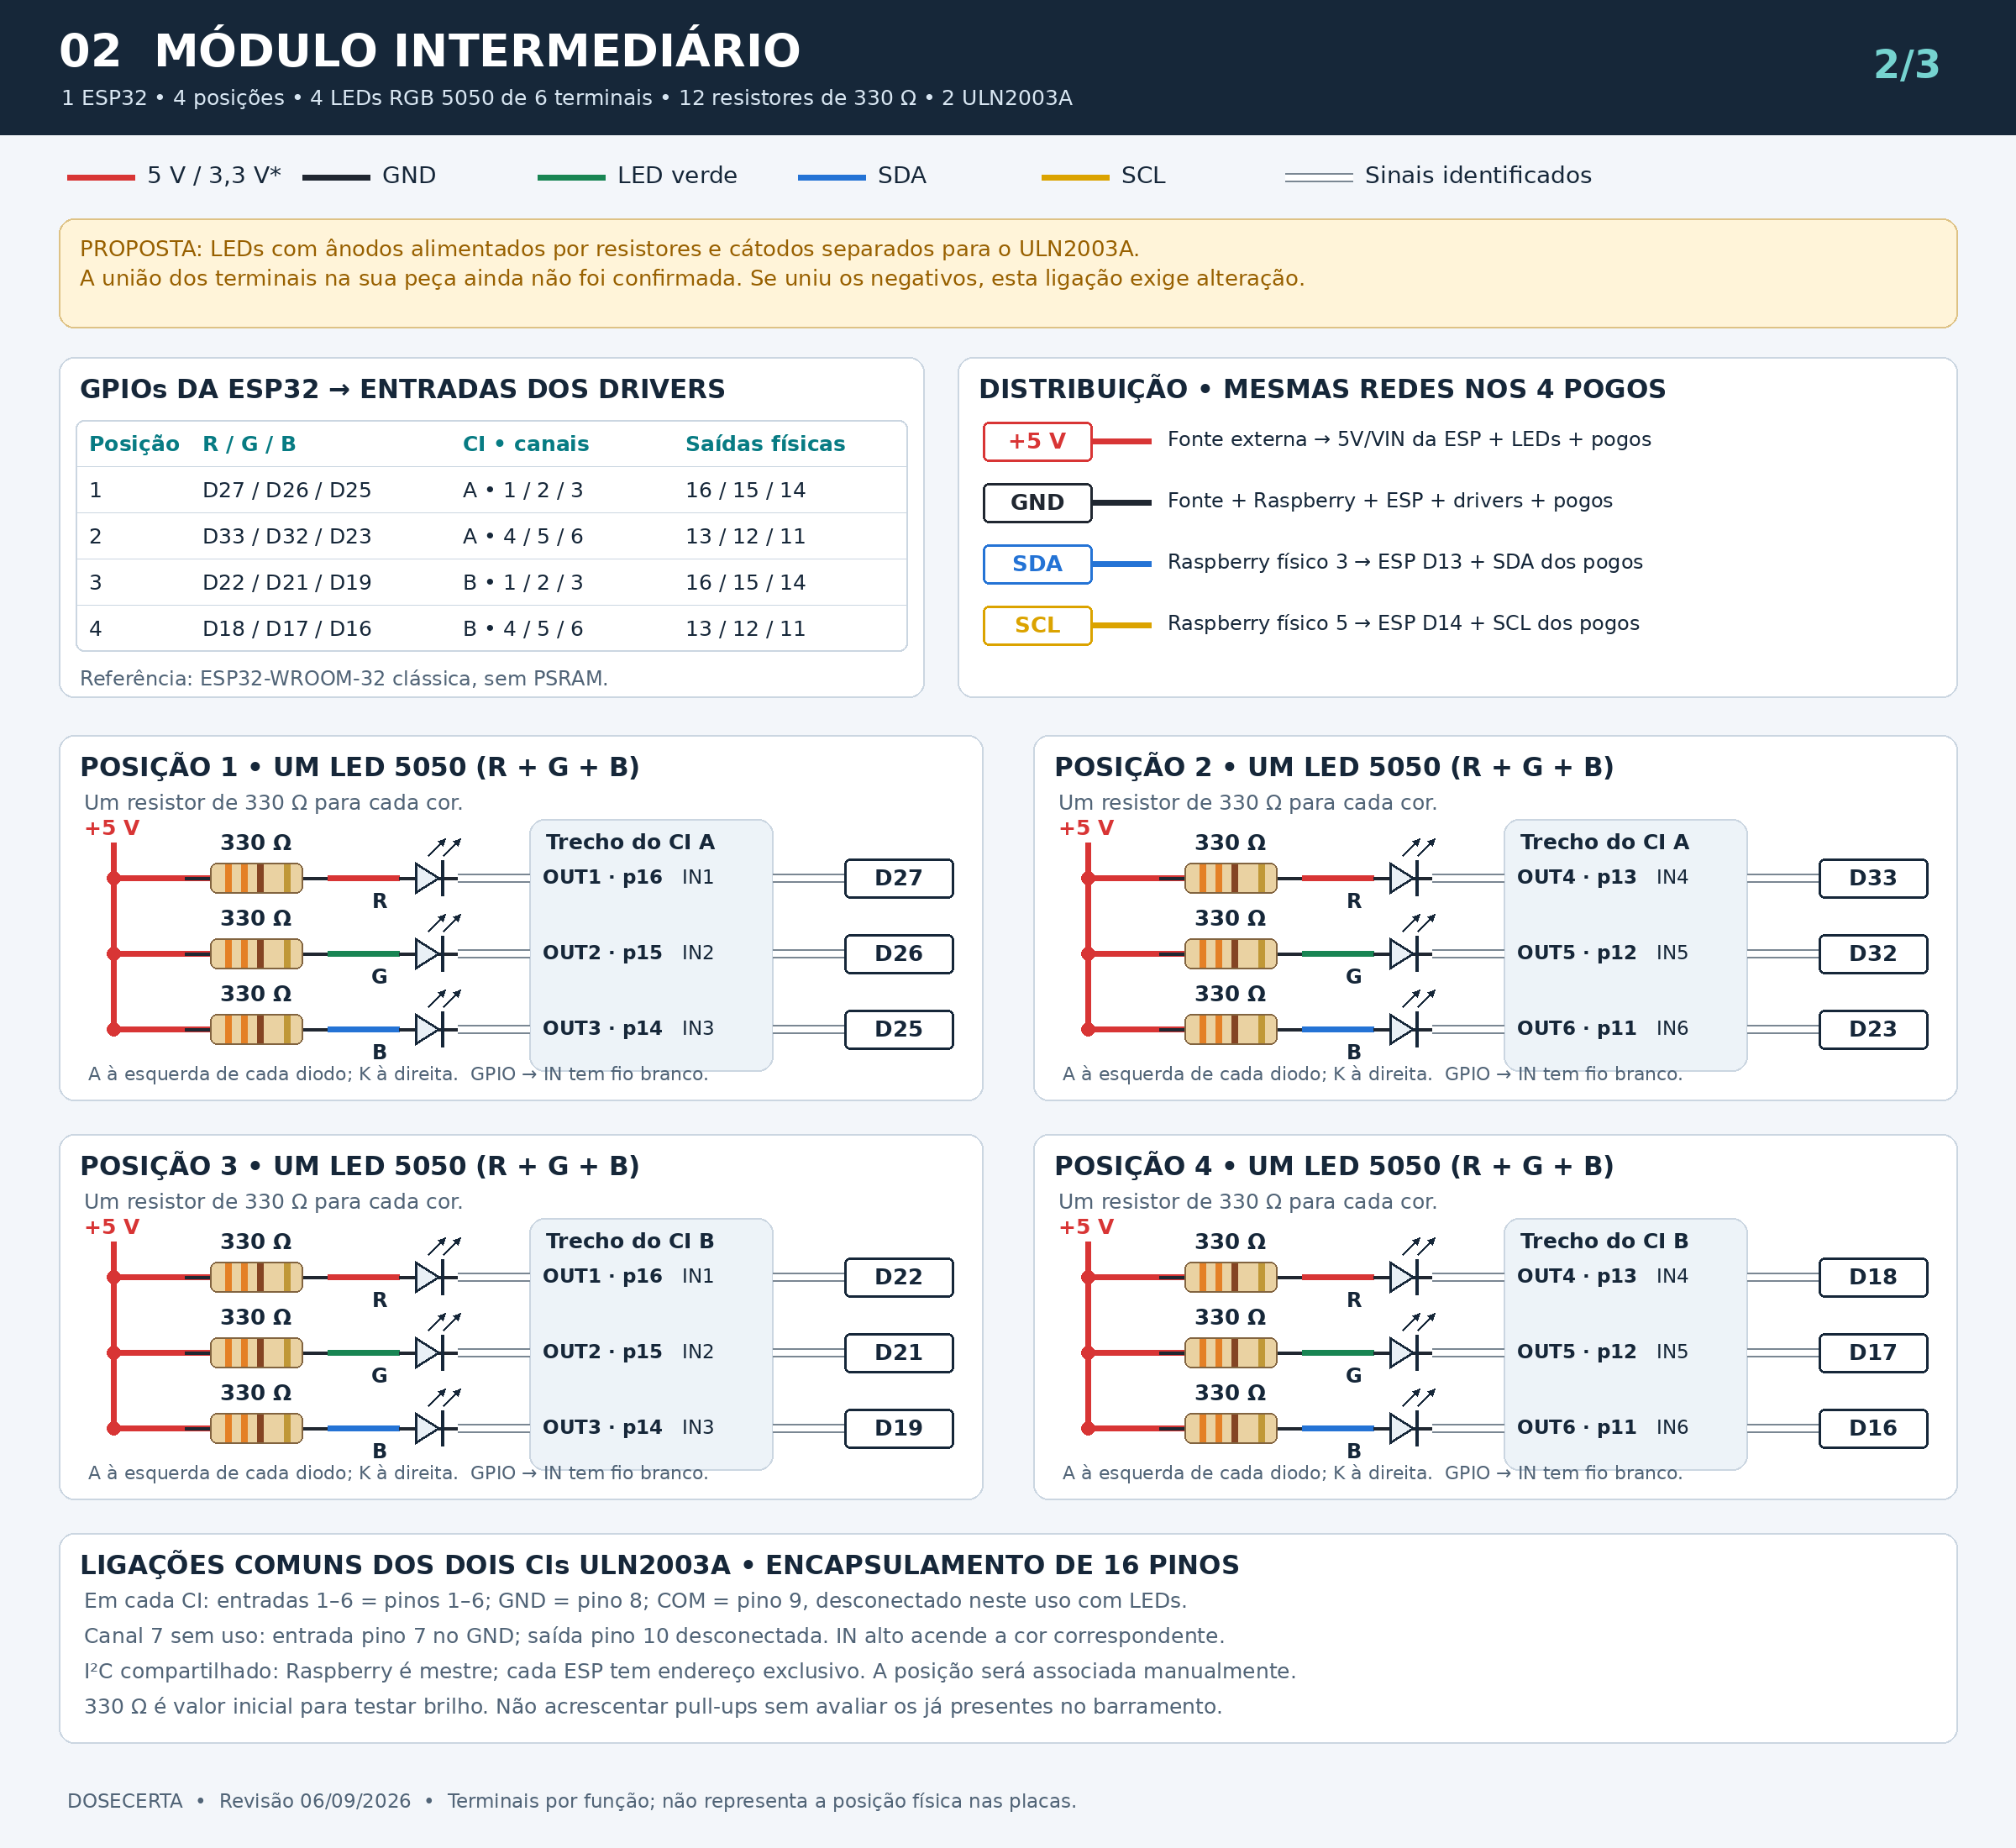
\includegraphics[width=0.98\textwidth,height=0.70\textheight,keepaspectratio]{Figuras/SharePoint/circuito_intermediario.png}
\fonte{Elaboração dos autores (set. 2026). Topologia a conferir na montagem final.}
\end{figure}


{\small\begin{longtable}{p{0.22\textwidth}p{0.22\textwidth}p{0.22\textwidth}p{0.22\textwidth}}
\caption{GPIO dos canais luminosos do intermediário}\label{tab:eletrica-gpio}\\
\hline\textbf{Canal} & \textbf{Vermelho} & \textbf{Verde} & \textbf{Azul}\\\hline\endfirsthead
\hline\textbf{Canal} & \textbf{Vermelho} & \textbf{Verde} & \textbf{Azul}\\\hline\endhead
L1 & 27 & 26 & 25\\\hline
L2 & 33 & 32 & 23\\\hline
L3 & 22 & 21 & 19\\\hline
L4 & 18 & 17 & 16\\\hline
\end{longtable}\noindent Fonte: projeto elétrico dos autores.\par}

A disposição dos encaixes e dos canais é mostrada na Figura~\ref{fig:encaixes_intermediario}. Cada posição fica entre dois LEDs, permitindo identificá-la pelo par adjacente. Assim, a confirmação visual de uma posição não depende de um LED instalado no submódulo.

\begin{figure}[htbp]
\centering
\caption{Disposição funcional dos encaixes e canais luminosos do intermediário}\label{fig:encaixes_intermediario}
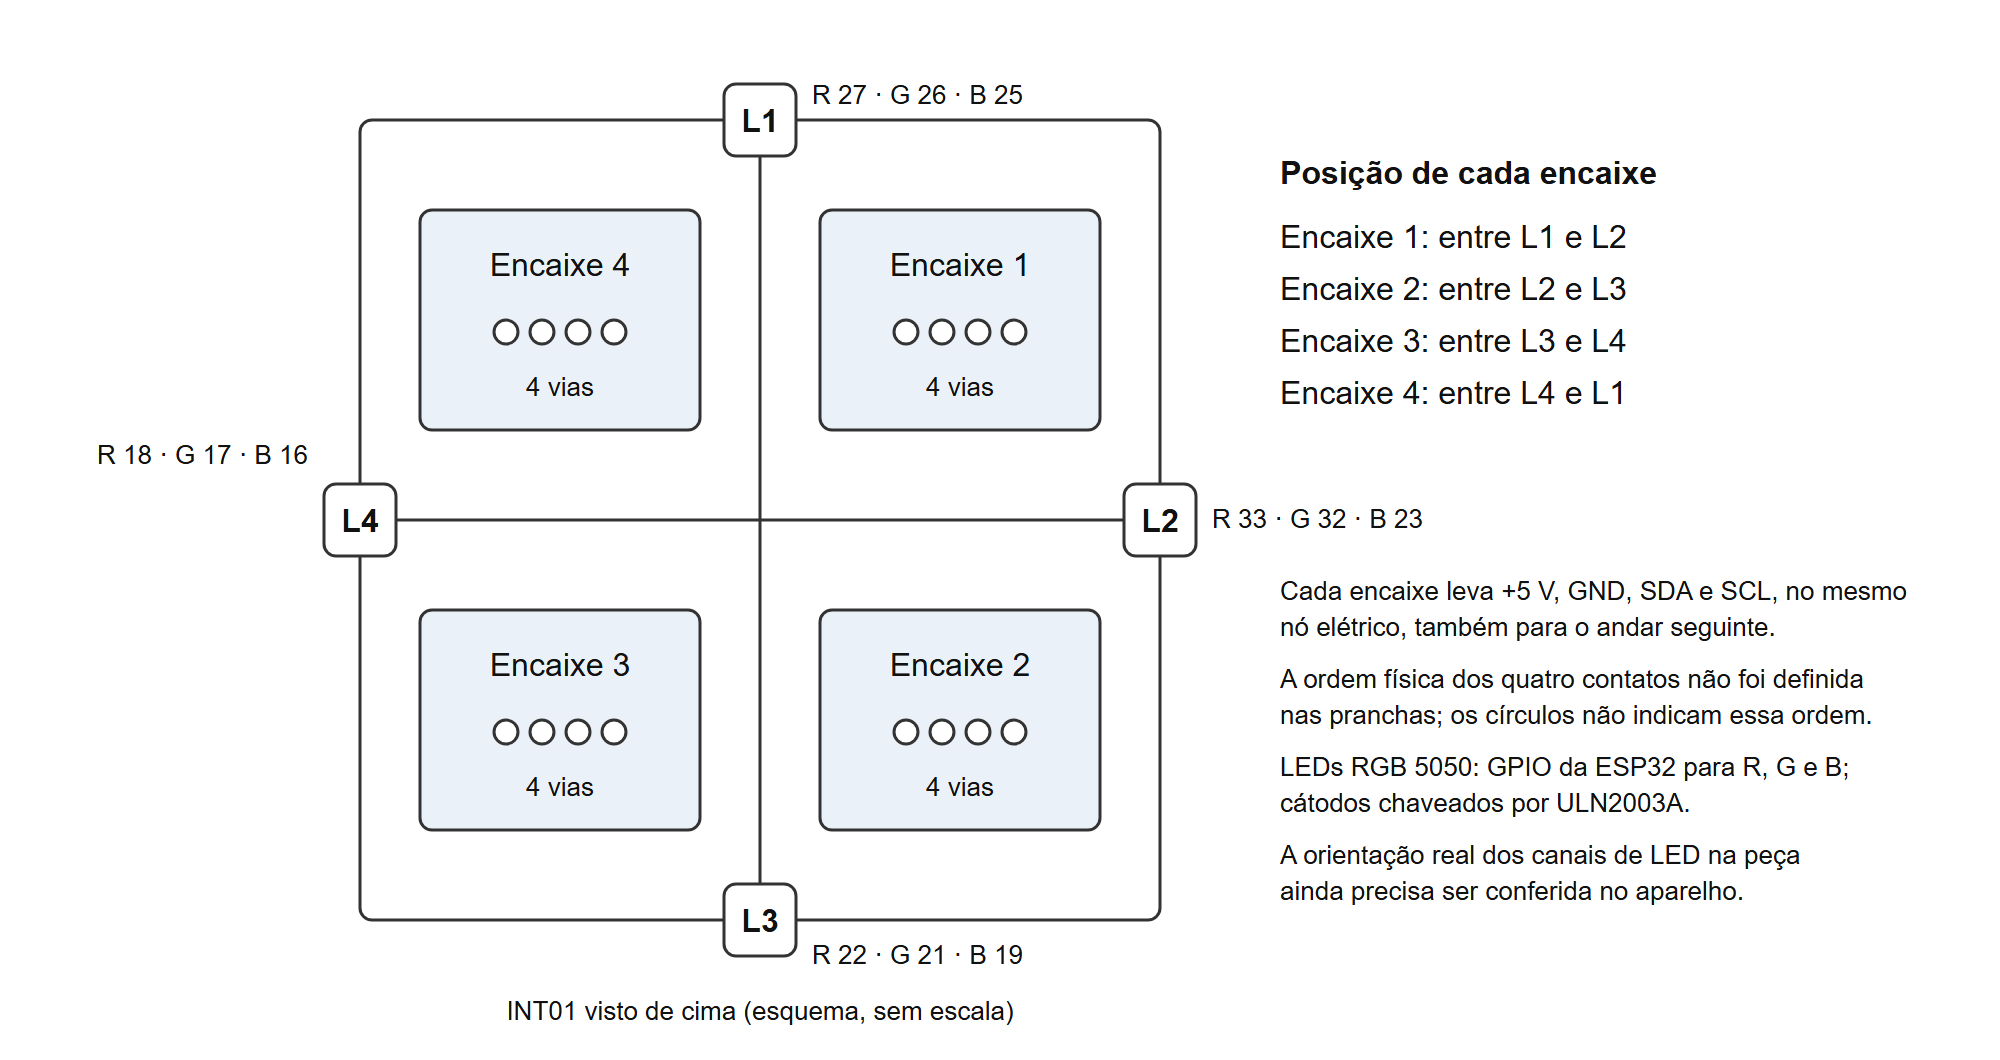
\includegraphics[width=0.98\textwidth,height=0.66\textheight,keepaspectratio]{Figuras/SharePoint/encaixes_intermediario.png}
\fonte{Elaboração dos autores (2026).}
\end{figure}


\section{Barramento, contatos e verificações}
As vias de alimentação e comunicação atravessam os encaixes no mesmo nó elétrico. Os níveis das linhas SDA e SCL devem permanecer compatíveis com a lógica de 3,3 V; resistores em paralelo e capacitância da montagem alteram os tempos de subida. O ensaio dos contatos inclui continuidade, resistência e estabilidade durante inserção e remoção, especialmente porque o requisito prevê modularidade com o equipamento energizado.

A seleção de capacitores, proteções e condutores deve considerar a montagem final. A avaliação de tensão no ponto de carga e de comportamento durante o motor fornece a base para esses ajustes. As pranchas apresentadas descrevem a distribuição funcional e devem permanecer vinculadas à revisão da fiação ensaiada.

\section{Orçamento dos componentes}
As planilhas de aquisição e de proposta utilizam bases distintas. A lista XLSX totaliza R\$ 2.494,305, mantidas três casas decimais para rastreabilidade; a proposta XLSM e o contrato registram R\$ 2.499,89. A Tabela~\ref{tab:08-3} apresenta os totais por item de cada planilha. Esses valores são orçamentos, não despesas comprovadas. \cite{DC_LISTA,DC_PROPOSTA,DC_CONTRATO}

{\small\setlength{\tabcolsep}{3pt}\begin{longtable}{p{0.43\textwidth}p{0.07\textwidth}p{0.17\textwidth}p{0.17\textwidth}}\caption{Lista de aquisição: valores totais por item em cada planilha}\label{tab:08-3}\\
\hline
\textbf{Item} & \textbf{Qtd.} & \textbf{XLSX (R\$)} & \textbf{XLSM (R\$)}\\\hline
\endfirsthead\hline
\textbf{Item} & \textbf{Qtd.} & \textbf{XLSX (R\$)} & \textbf{XLSM (R\$)}\\\hline
\endhead
ESP32 & 10 & 407,500 & 407,500\\\hline
Motor De Passo 28byj-48 + Driver Uln2003 & 9 & 110,700 & 110,700\\\hline
PLA Branco 1KG & 5 & 422,750 & 450,000\\\hline
Raspberry Pi Zero 2W & 1 & 542,000 & 548,000\\\hline
Módulo de câmera Raspberry Pi 3 & 1 & 580,000 & 580,000\\\hline
Kit 100 de imãs & 1 & 32,000 & 32,000\\\hline
Parafuso Philips Cabeça Chata Inox M3x6mm & 10 & 1,800 & 1,800\\\hline
Parafuso Philips Cabeça Chata Inox M3x12mm & 10 & 2,400 & 2,400\\\hline
Parafuso Philips Cabeça Chata Inox  M3x16mm & 10 & 14,200 & 14,200\\\hline
Porca M3 & 30 & 3,300 & 3,300\\\hline
10 LED RGB WS2812B 5050 & 1 & 6,000 & 6,000\\\hline
Fonte De Alimentação 5v 10a & 1 & 49,990 & 49,990\\\hline
Fretes & 1 & 94,910 & 94,000\\\hline
Diversos & 1 & 226,755 & 200,000\\\hline
\end{longtable}}{\small\noindent Fonte: Planilhas XLSX e XLSM fornecidas pela equipe; totais orçados, três casas decimais para rastreabilidade. O WS2812B pertence ao orçamento; a montagem documentada utiliza RGB 5050 comum de seis terminais, sem controlador integrado.\par}

A diferença entre as bases decorre de preços e arredondamentos presentes nos arquivos de origem. O custo da configuração efetivamente construída deve considerar quantidade instalada, substituições e comprovantes, sem converter automaticamente o orçamento em custo final.

\section{Correspondência com a montagem fotografada}
A Figura~\ref{fig:central_interna_2026} mostra o interior da central, a Raspberry Pi, o cabo da câmera e o módulo de relógio. A fotografia do RTC comprova sua presença física no conjunto registrado, mas não confirma habilitação, acerto nem manutenção do tempo após retirada da alimentação principal. \cite{DC_VALIDACAO2026}

\begin{figure}[htbp]
\centering
\caption{Interior da central: (a) conjunto aberto; (b) Raspberry Pi; (c) cabo da câmera; (d) módulo RTC e conexões}\label{fig:central_interna_2026}
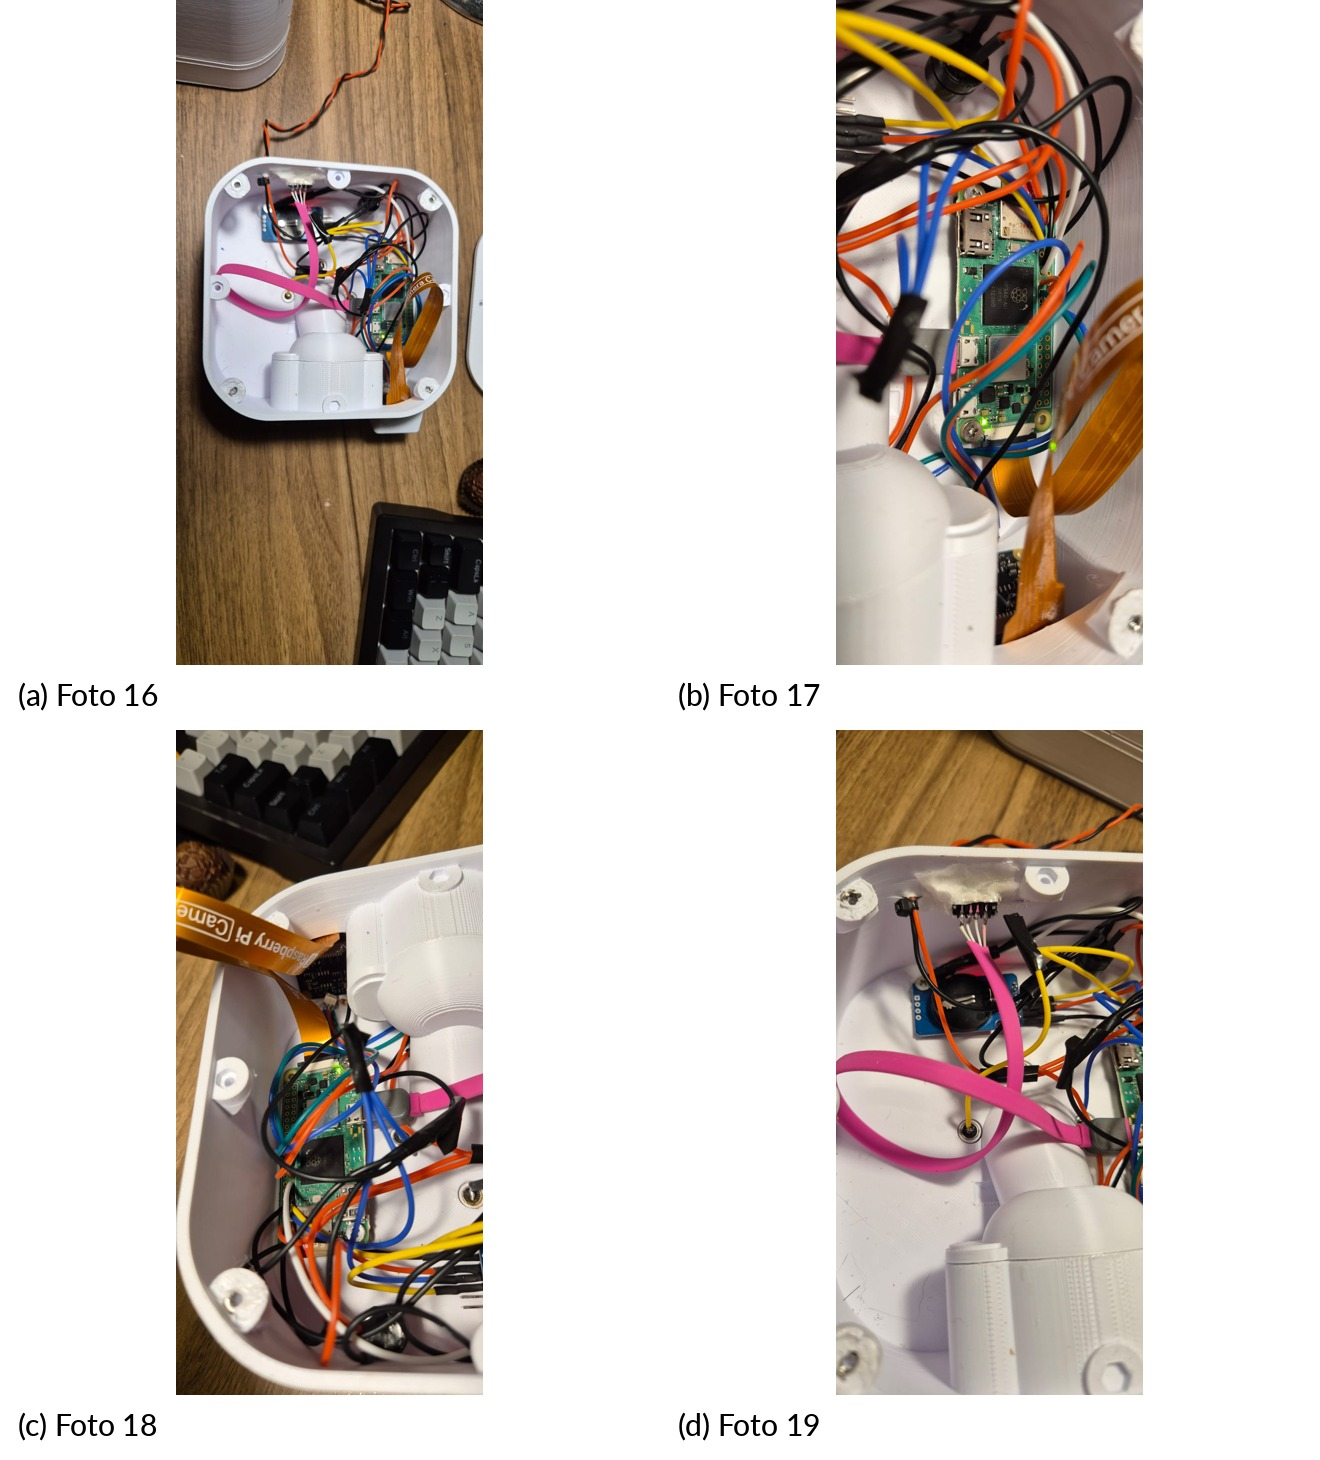
\includegraphics[width=0.98\textwidth,height=0.69\textheight,keepaspectratio]{Figuras/Validacao20261126/central_eletronica.jpg}
\fonte{Acervo dos autores, pacote de validação recebido em novembro de 2026.}
\end{figure}

As Figuras~\ref{fig:int_fisico_2026} e~\ref{fig:int_chicote_2026} permitem relacionar os encaixes, indicadores e chicote à descrição funcional. O I²C comum identifica a placa, não a posição física do encaixe; a associação continua dependente de cadastro e confirmação humana. A orientação dos canais não foi deduzida das cores aparentes nas fotos.

\begin{figure}[htbp]
\centering
\caption{Intermediário: (a) cavidades de encaixe; (b) contatos superiores; (c) LEDs verdes; (d) submódulo encaixado com LEDs azuis}\label{fig:int_fisico_2026}
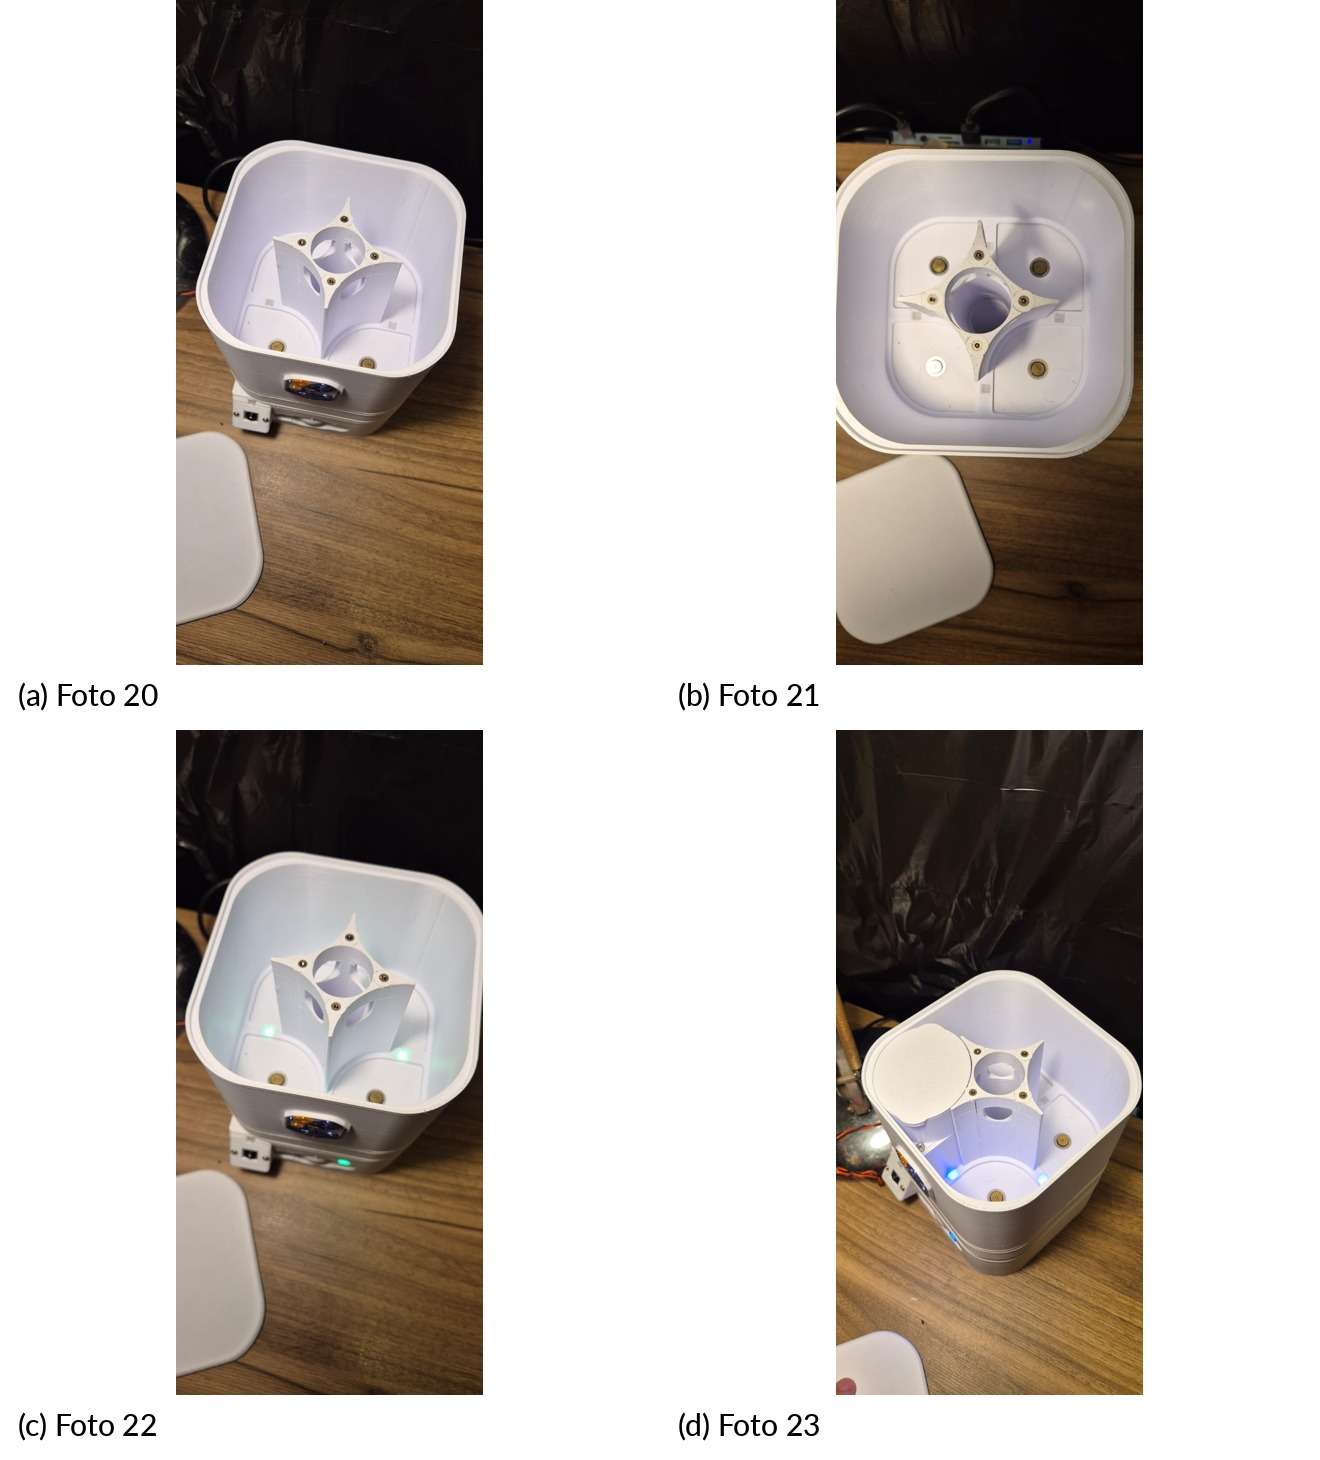
\includegraphics[width=0.98\textwidth,height=0.69\textheight,keepaspectratio]{Figuras/Validacao20261126/intermediario.jpg}
\fonte{Acervo dos autores, pacote de validação recebido em novembro de 2026.}
\end{figure}

\begin{figure}[htbp]
\centering
\caption{Intermediário aberto: (a) submódulo no encaixe; (b) chicote; (c) contatos e ligações inferiores}\label{fig:int_chicote_2026}
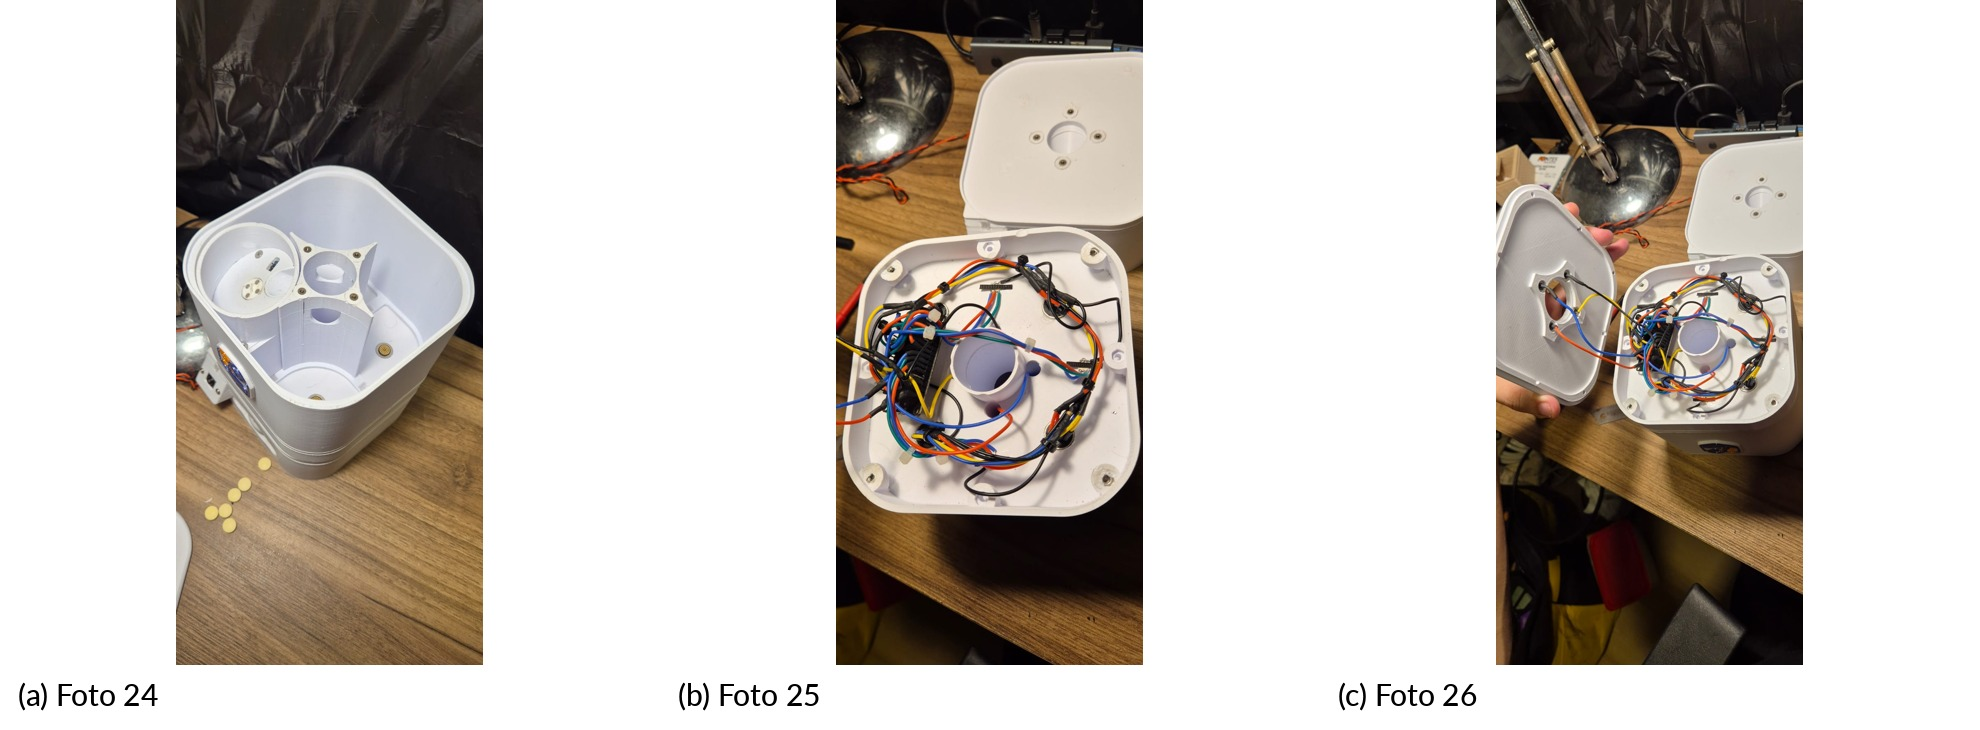
\includegraphics[width=0.98\textwidth,height=0.69\textheight,keepaspectratio]{Figuras/Validacao20261126/intermediario_chicote.jpg}
\fonte{Acervo dos autores, pacote de validação recebido em novembro de 2026.}
\end{figure}

A Figura~\ref{fig:sub_eletronica_2026} documenta ESP32, motor e placa de acionamento do submódulo. Esses registros vinculam a descrição aos componentes montados, sem substituir medições de tensão, corrente ou temperatura sob carga.

\begin{figure}[htbp]
\centering
\caption{Eletrônica do submódulo: (a) motor e driver; (b) ESP32; (c) conjunto 28BYJ-48 e interface de potência}\label{fig:sub_eletronica_2026}
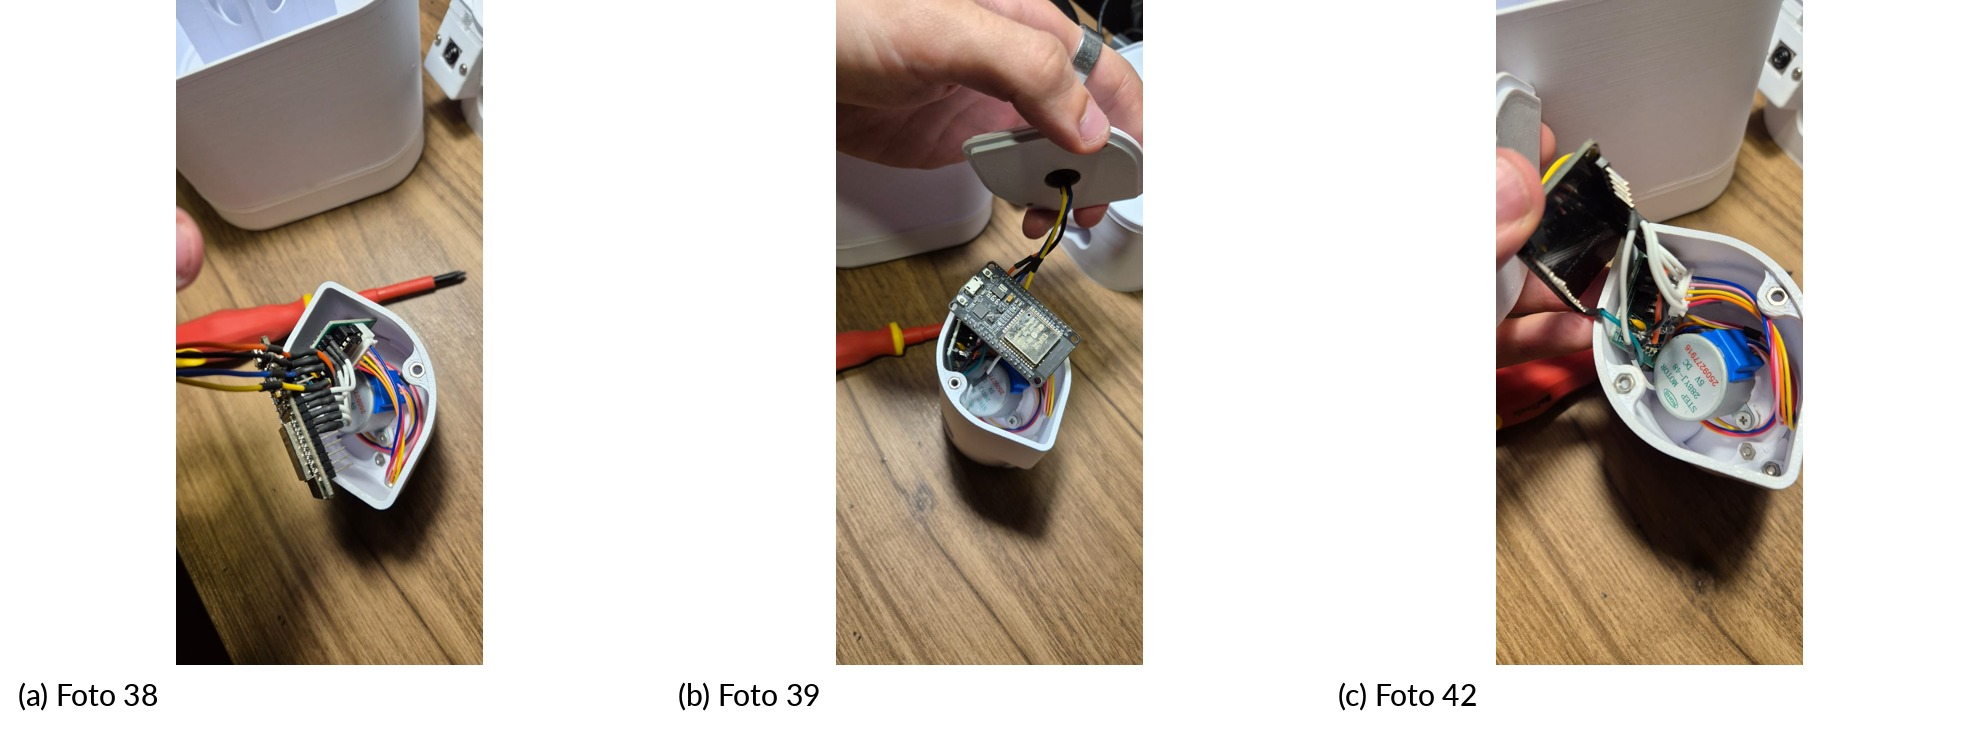
\includegraphics[width=0.98\textwidth,height=0.69\textheight,keepaspectratio]{Figuras/Validacao20261126/sub_eletronica.jpg}
\fonte{Acervo dos autores, pacote de validação recebido em novembro de 2026.}
\end{figure}

\section{Leituras posteriores e limites do diagnóstico elétrico}
Em novembro houve nova perda de comunicação do submódulo durante movimento após os reparos de fiação. O motivo de reinício dessa ocorrência não foi recuperado antes do reencaixe; não se pode atribuí-la conclusivamente ao mesmo brownout do primeiro registro. A recomendação de medir os 5 V junto ao SUB01 durante o giro e avaliar desacoplamento de 470~$\mu$F e 100~nF permanece uma ação de diagnóstico, não uma correção cuja montagem e eficácia estejam demonstradas. \cite{DC_VALIDACAO2026}

Na coleta de 26 de novembro, INT01 e SUB01 voltaram a responder e a telemetria sem motor não mostrou mudança de boot nas amostras válidas. A central ficou entre 53,69~°C e 57,46~°C; as leituras do indicador \texttt{get\_throttled} foram zero. Esses dados descrevem a condição monitorada da Raspberry, não a temperatura de todos os componentes nem a tensão transitória nos contatos. Não substituem ensaio elétrico com carga. \cite{DC_VALIDACAO2026}

\section*{\textcolor{DCPendente}{Complementações necessárias}}
\pendencia{ELE01}{Informar marca/modelo da fonte instalada, etiqueta, regulação, fusíveis, aterramento, proteção e cabeamento. Medir tensão na Pi e nos módulos, queda de tensão, corrente em repouso/atuação e aquecimento. Não tratar 10 A como consumo.}
\pendencia{ELE02}{Conferir ordem, orientação e continuidade real de cada pogo, comprimentos, bitolas e retornos. Completar esquema elétrico pós-reparos e identificar conectores por modelo ou desenho cotado.}
\pendencia{ELE03}{Medir pull-ups equivalentes, capacitância/tempos de subida e níveis do I²C com os módulos e os motores; verificar colisão de endereços, taxas de erro e comportamento no encaixe/retirada energizados. O mapa funcional não atesta integridade elétrica.}
\pendencia{ELE04}{Conferir pinagem do TCRT5000 físico, resistores, alimentação e faixa ADC; obter leituras em cavidade vazia/ocupada e sob diferentes condições. Medir comportamento do motor, driver e sensor em conjunto, sem confundir leitura da cavidade com sensor de saída.}
\pendencia{ELE05}{Confirmar LED adquirido/instalado, terminais A/K, corrente e brilho por cor, resistores e dissipação dos drivers. Fornecer fotos e testes de todas as posições; não assumir funcionamento dos dois intermediários a partir de uma unidade.}
\pendencia{ELE06}{Identificar RTC e bateria realmente instalados; conferir carga e compatibilidade da placa, habilitação no Linux, leitura de /dev/rtc0 e teste após desligamento sem rede. A bateria do RTC não alimenta a Pi.}
\pendencia{ELE07}{Fechar ensaios de buzzer, LEDs centrais, chaveamento, aquecimento, reinício e interferência em conjunto. Inserir esquema final, registros dos instrumentos e condições; confirmar capacitores/proteções acrescentados nos reparos.}
\pendencia{BOM01}{Conciliar os orçamentos XLSX e XLSM/contrato com compras, doações e fretes; o valor anterior de R\$ 2.512,55 não foi localizado e não é adotado. Não preencher custo realizado com orçamento.}
\pendencia{BOM02}{Completar a lista técnica instalada com sensores, conectores pogo, resistores, drivers de LEDs, buzzer/MOSFET, RTC, bateria, cabos, proteções e demais itens. Conferir a troca de WS2812B cotado pelo RGB comum documentado.}
